\section{Results and Tests}

\subsection{Testing functionality}
We tested that our application worked as it should by observing how the system reacted to button press on the gamepad. The buttons have the following defined behaviour:
\begin{itemize}
	\item \emph{Button 1} - No action. 
	\item \emph{Button 2} - Change to sawtooth waveform.
	\item \emph{Button 3} - Change to triangle waveform.
	\item \emph{Button 4} - Change to square waveform.
	\item \emph{Button 5} - Play Tetris Theme Song, our startup melody.
	\item \emph{Button 6} - Play Star Wars Imperial March.
	\item \emph{Button 7} - Play sound effect 1.
	\item \emph{Button 8} - Play sound effect 2.
\end{itemize}

We could indeed confirm that buttons 5-8 played the auido we expected. \\
\\
When we tested the different waveforms (button 2, 3 and 4), none of us had any idea what the different waves would sound like. We observed that the audio sounded differently (more or less metallic), but still correct (as described in \ref{audio_correctness}). We therefore concluded that waveform selection functionality was working properly.

\subsubsection{Audio correctness and quality}
\label{audio_correctness}
We have no knowledge of how to scientifically test the audio correctness and quality, so we used our own ears. We accepted the music and sound effects if they "sounded allright". By that we mean that all the tones in the audio was pure, playing in the correct tempo and having the expected pitch. 

\begin{figure}[h]
	\centering
	\begin{tabular}{c | c  c}
			& Tetris Theme Song & Idle \\
		\hline
		\hline
		High frequency timer & $4.628mA$ & $4.990mA$ \\
		Low frequency timer & $2.980mA$ & $1.213mA$ \\
		Energy Mode 3 when idle & $2.988mA$ & $0.213mA$ \\

	\end{tabular}
	\caption{Average amperage in different modes.}
	\label{fig:energy_results}

\end{figure}

\subsection{Testing energy efficiency}
During the development of the system, we tested the energy efficiency using the \emph{energyAware Profiler}. We recorded the amperage at two different situations; when the system was playing the three tracked Tetris Theme Song and when it was idle. The results can be found in figure \ref{fig:energy_results}. \\
\\
The results were as expected, and we are satisified that our final solution only has an average power consupmtion of $0.213mA$ when idle (Energy Mode 3). Turning off the low frequency oscilators when idle gave us five times better energy efficiency; having interrupts generated 32,000 times a second is costly.\\
\\
Although using the low frequency timers forced us to reduce the sampling rate from $48kHz$ to $32kHz$, we observed that the amperage when playing the Tetris Theme Song is close to half with the low frequency timers. Here, we see a tradeoff between energy effectiveness and audio quality. We chose the energy effective solution, as $32kHz$ was enough for the audio we are generating.

\begin{figure}[hf]
	\centering
	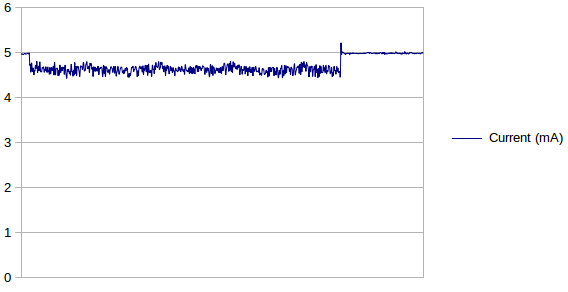
\includegraphics[width=8cm]{img/hf.png}
	\caption{High frequency timer energy consumption.}
	\label{fig:hf}
\end{figure}
	
\begin{figure}[hf]
	\centering
	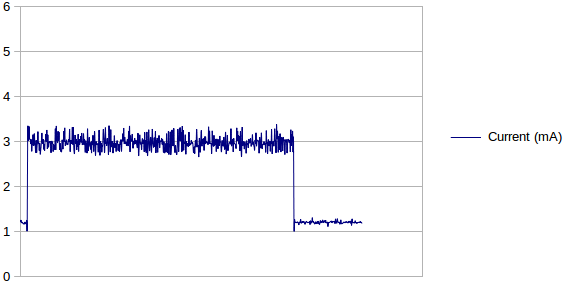
\includegraphics[width=8cm]{img/em3.png}
	\caption{Energy Mode 2 energy consumption.}
	\label{fig:em3}
\end{figure}

\begin{figure}[hf]
	\centering
	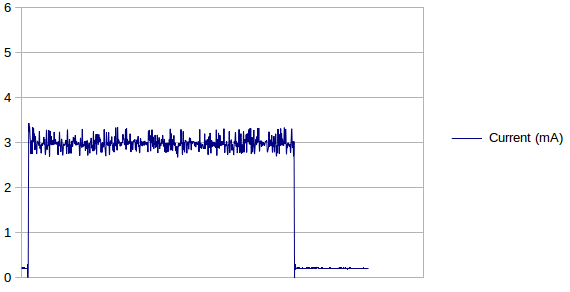
\includegraphics[width=8cm]{img/em3_sleep.png}
	\caption{Energy Mode 2 (3 when idle) energy consumption.}
	\label{fig:em3_sleep}
\end{figure}
\subsection{Discussion - Room for improvements?}

